\begin{tikzpicture}[-{Latex[length=1.5mm]}]
  \onslide<1->{\node[inner sep=0pt] (cell) {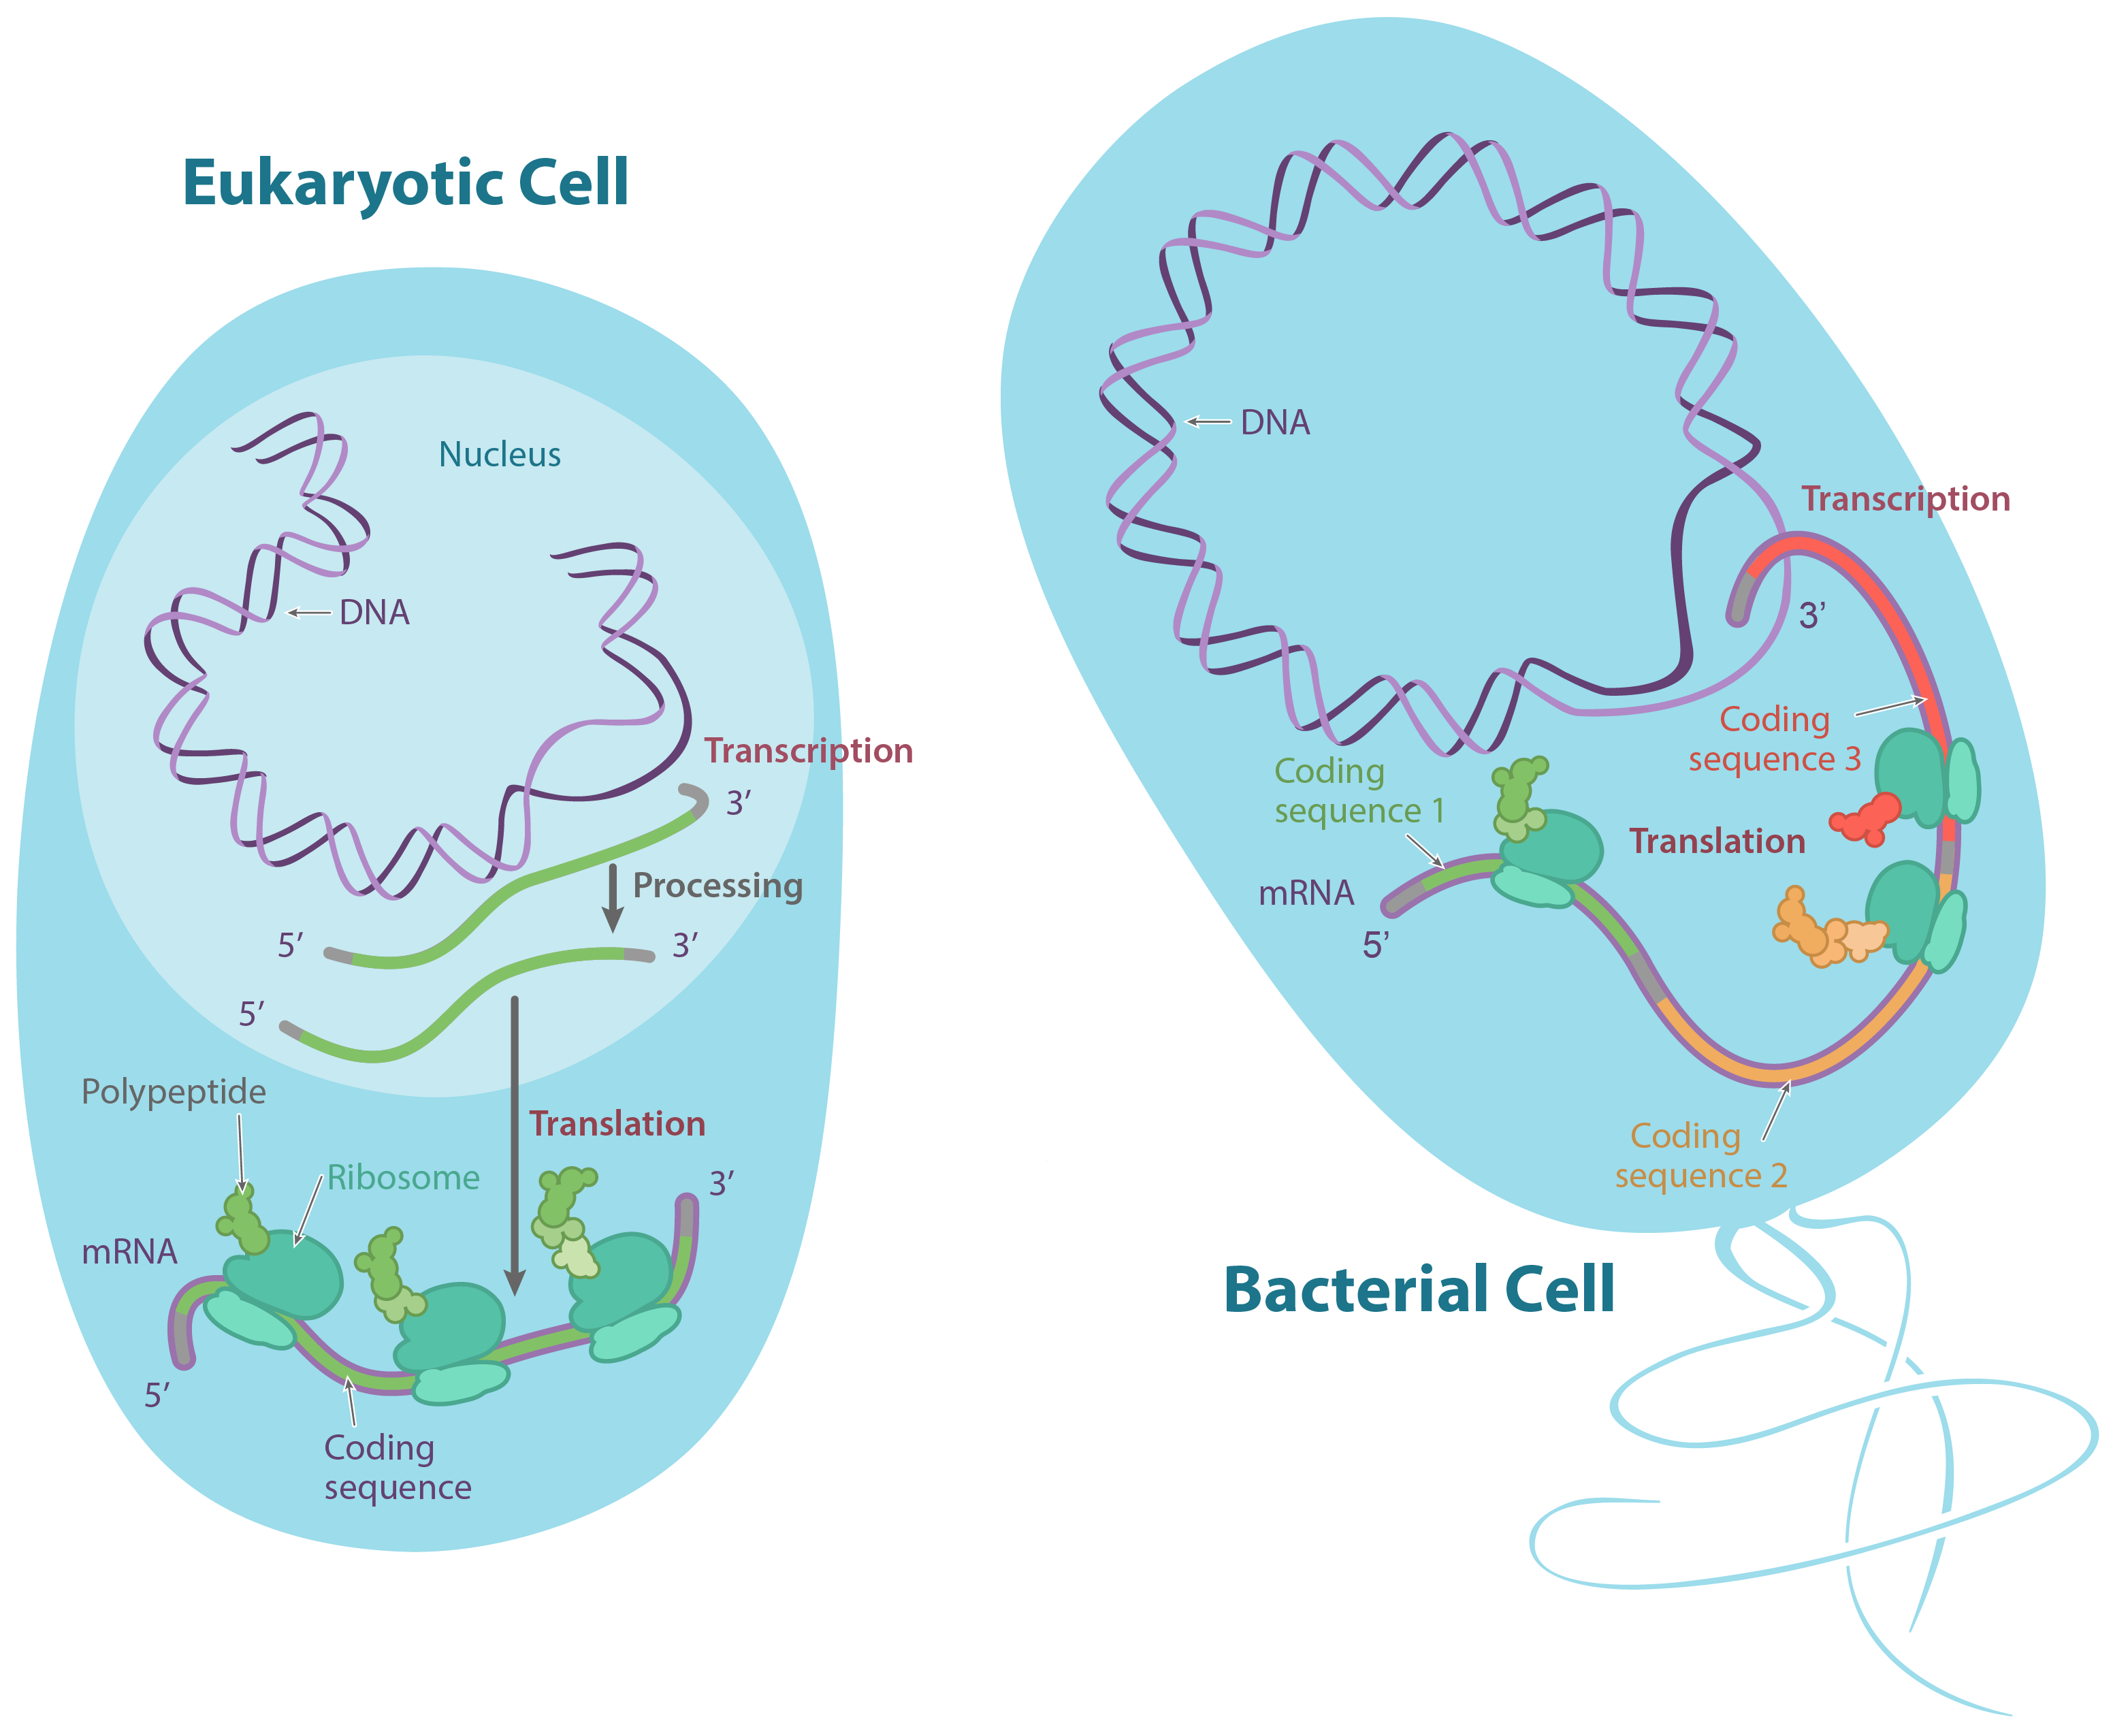
\includegraphics[width=0.45\textwidth]{cell.png}};}
  \onslide<3->{\node[right = of cell] (rnaA)  {\scriptsize RNA of $a$};}
  \onslide<2->{\node[above = of rnaA] (dnaA) {\scriptsize DNA of gene $a$};}
  \onslide<1->{\draw[-latex,thick] (cell) -- (rnaA);}
  \onslide<4->{\node[below = of rnaA] (prA) {\scriptsize Protein of $a$};}
  \onslide<2->{\node[right = of dnaA] (dnaB) {\scriptsize DNA of gene $b$};}
  \onslide<5->{\node[below = of dnaB] (rnaB) {\scriptsize RNA of $b$};}
  \onslide<6->{\node[below = of rnaB] (prB) {\scriptsize Protein of $b$};}
  \onslide<3->{\draw (dnaA) to (rnaA);}
  \onslide<4->{\draw (rnaA) to (prA);}
  \onslide<5->{\draw (dnaB) to (rnaB);}
  \onslide<6->{\draw (rnaB) to (prB);}
  \onslide<10->{\node[draw,dotted,fit=(dnaA) (rnaA) (prA),label=above:$a$] (entityA){};}
  \onslide<11->{\node[draw,dotted,fit=(dnaB) (rnaB) (prB),label=above:$b$] (entityB){};}

  \onslide<7->{\draw[bend right=15, color=blue!50] (prB) to (dnaA);}
  \onslide<8->{\draw[-|,bend left=15,color=red] (prA) to (dnaB);}
  %\onslide<9->{\draw[bend right=45, color=blue!50,dashed] (prB) to (dnaB);}
\onslide<13->{
\node (a) [draw,circle,below left = 2cm and 1cm of entityA] {$a$};
\node (b) [draw,circle,right = of a] {$b$};
\draw[-{Latex[length=1.5mm]}, line width=1pt] (a) to[bend left] (b);
\path (b) edge[-|,thick,bend left=30,shorten >=1pt] (a);
%\draw[-{Latex[length=1.5mm]}, thick, loop above,dashed] (b) to (b);
}
\node[fit=(a)(b)](mid){};
\onslide<12->{\draw[-latex,thick] (prA) -- (mid);}
\onslide<14->{\node [draw=none, right = of b]{How to compute with BRN?};}
\end{tikzpicture}